\chapter{Implementation}

This chapter presents the decisions and selected approaches for implementation, intending to give an overview of what the application does and how one conducts rendering.
One wants to illustrate the complexity of a path tracer and define goals and potential problems.

The thesis aims to create a path tracer with the Disney illumination model so that one can analyse the illumination model whilst having maximum control over the path tracer.
The requirements are that the path tracer can render images \textit{fast} and that the source code is \textit{understandable}.
Having something fast and understandable becomes tricky; therefore, one must make compromises.

As explained earlier, path tracing can become computationally expensive.
The expense is because of three factors: path construction process, pixel samples, and light calculations.
Depending on how one defines these factors, they pose a problem for \textit{fast} path tracing.

One has to utilise two powerful tools: a ray tracing library and parallel computing.
To give some context, let one first illustrate the necessity for parallelism and then elaborate on ray tracing libraries.

\section{Parallelism}

Now, one gives a rough insight into parallelism, what it means and why it is relevant for path tracing.

The field of parallel computing to enable parallelism has become essential in computer science over the last decades as hardware performance does not follow Moore's law anymore; \cite{theis_end_2017}.
For clarification, one specifies the term \textit{parallelism}.
It describes the proper simultaneous execution of two distinct instruction streams; \cite{laplante_encyclopedia_2017}.
In other words, hardware with more than one execution unit (processing core) can simultaneously execute multiple tasks.
Accordingly, introducing multi-core central processing units (CPU) qualifies for parallelism but in a narrow scope.
However, one should remember that manufacturers have optimised CPUs for serial processing, unlike the graphics processing unit (GPU).
GPUs are specialised for a high throughput of tasks by providing many cores and threads for execution.
If an application exhibits data-level parallelism, these processors accelerate; \cite{laplante_encyclopedia_2017}.

One defines path tracing as an application with data-level parallelism because the path construction process qualifies for independent path calculations.
Note that data management, underlying algorithms and data structures, and particular hardware acceleration determine the degree of parallelism.
For the following, one assumes that GPUs allow a level of parallelism in order of magnitudes, which results in a performance increase.

\section{Ray Tracing Libraries}

Ray Tracing libraries offer generic tools to execute ray tracing efficiently \cite{nvidia_nvidia_2022}, \cite{intel_embree_2022}, \cite{khronos_vulkan_2022}, \cite{microsoft_directx-spec_2022}.
They are available for a processor and a graphics card implementation.
The fact that makes these libraries unique is that they have state-of-the-art algorithms and data structures optimally implemented to reduce processing time whilst providing great flexibility because of a  programmable pipeline.
This pipeline has a predefined procedure where one can program components to define custom logic and behaviour.
Additionally, the libraries tend to be verbose and expose technical details, making the handling of the libraries less intuitive but allowing for more refined controls.

One further simplifies the selection process by assuming that the choice of a ray tracing library has little to no performance impact because the algorithms and data structures can be virtually equivalent; \cite{bico_optix_2016}.

\section{Tools}

Finally, one can decide upon the various tools available to implement a path tracer with the Disney illumination model.
To make the decision-making more reasonable, one gives an example demonstrating the difficulties of rendering.

One would like to render a scene with multiple triangles meshes that totalled a million triangles.
The image should have a resolution of 1024x1024 pixels with one hundred twenty-eight samples per pixel, and one has constructed the scene in a way that paths have exactly three vertices and two segments on average.

At first glance, it seems like a trivial task.
Nonetheless, one analyses the example by breaking it into parts, beginning with the triangle meshes.
As one maybe knows, intersection tests for every triangle in the scene is a computationally expensive action.
Because of this, one utilises a ray tracing library offering an acceleration structure that reduces the number of tests and thus makes rendering \textit{faster}.
In recent years, GPU manufacturers extended hardware with special-purpose components for ray tracing or machine learning, another factor that increases performance for these tests.
Because of that, it makes the hardware undeniably computationally faster for these purposes, making a GPU already a preferred choice.
Next, one will examine the image resolution, sample count and path calculations (\ref{sec:path-tracing}).
These three metrics are driving factors determining the number of operations necessary to calculate the image.
An operation, in this context, is an abstract unit resembling something like a floating-point calculation on a processing unit.
Besides, one supposes that a ray cast and the light calculations at a vertex count separately as one operation to simplify the estimation.
With the current example, one has about a million pixels and one hundred twenty-eight samples per pixel, requiring the application to calculate one hundred twenty-eight million paths.
Accordingly, one must find these paths' vertices and segments, resulting in four operations per path and a billion operations in total.

Due to such scenarios, one decided to have GPU implementation because it qualifies for massively parallel computation.
In addition, ray tracing libraries have excellent GPU support.
The most promising benefit of a GPU implementation is the development feedback loop.
A flexible feedback loop is crucial because it enables one to render multiple images in a shorter time, making further image comparison more accessible.
Accordingly, it assists in an analysis of a series of images.
Another benefit is that one can increase the sample count without waiting hours to finish rendering an image, resulting in more iteration during the implementation.
On the opposite side, one has to consider the pitfalls of GPU programming and the libraries' verbose API.
First, development support concerning GPU programming is quite limited regarding general practices like debugging and unit testing.
The other part is the verbosity which introduces more complexity during development.
Nonetheless, the second requirement is the comprehensibility of the source code.

To partially circumvent the pitfalls, one demands another layer of abstraction, a wrapper library for the ray tracing libraries, simplifying the usage.
Furthermore, one will use the C++ programming language for the application due to a wide range of additional libraries and optional controls.
Note that selecting a ray tracing library where the GPU-sided programming is similar to the syntax of C++ helps with the source code's coherence.

The so-called OptiX Wrapper Library (OWL) is a library that satisfies the new demands, which indirectly selects OptiX as the ray tracing library.
Because of the wrapper, data access and function calls of OptiX are more straightforward.
The used programming language is CUDA, a \textit{subset} of the C++ language supporting most language features.
In addition, it is feasible to target the GPU and CPU with the compilation of source code, theoretically allowing for hybrid implementations.

\begin{list}{-}{}
    \item CMake 3.22.0
    \item C++20 and CUDA 17
    \item CUDA Runtime 11.7
    \item OptiX Ray Tracing API (SDK 7.4.0)
\end{list}

\section{CUDA and OptiX}

For this section, one has to discuss general ideas and principles of CUDA and OptiX because of the OWL library.

First, one likes to sharpen the understanding of CUDA.
One will simplify the description because these are sufficient for the implementation.
The GPU programming model \cite{nvidia_cuda_2022} distinguishes between a host (CPU-sided application) and a device (GPU-sided application).
This model introduces a strict separation of source code, memory and execution.
However, both sides can transfer data over the bus connection to ensure communication.
Accordingly, the CPU-sided application must prepare data and upload it to the GPU so that it can process the data.
Besides, one has to begin the execution of the device, which is possible through special functions called kernels.
Kernels are callable from the host that causes the execution of device code $N$ times in parallel by $N$ different threads.
Hence, threads represent the execution of one kernel.
The abstraction of threads provides a primitive for parallel programming where every thread has a unique index.
Consequently, one can work with linear buffers and address distinct elements through the threads index.
Nonetheless, it requires caution because race conditions can still happen.

Now, one give a introduction to OptiX \cite{nvidia_nvidia_2022}.
NVIDIA states that OptiX 7 builds upon the CUDA technology to facilitate ray tracing.
The provided ray tracing pipeline is especially noteworthy because of the programmable component.
The components are called programs, encapsulating a code block that expresses the program's application-dependent behaviour.
Next, one will briefly present the vital program types and the usage of these programs.

\begin{figure}[h]
    \begin{center}
        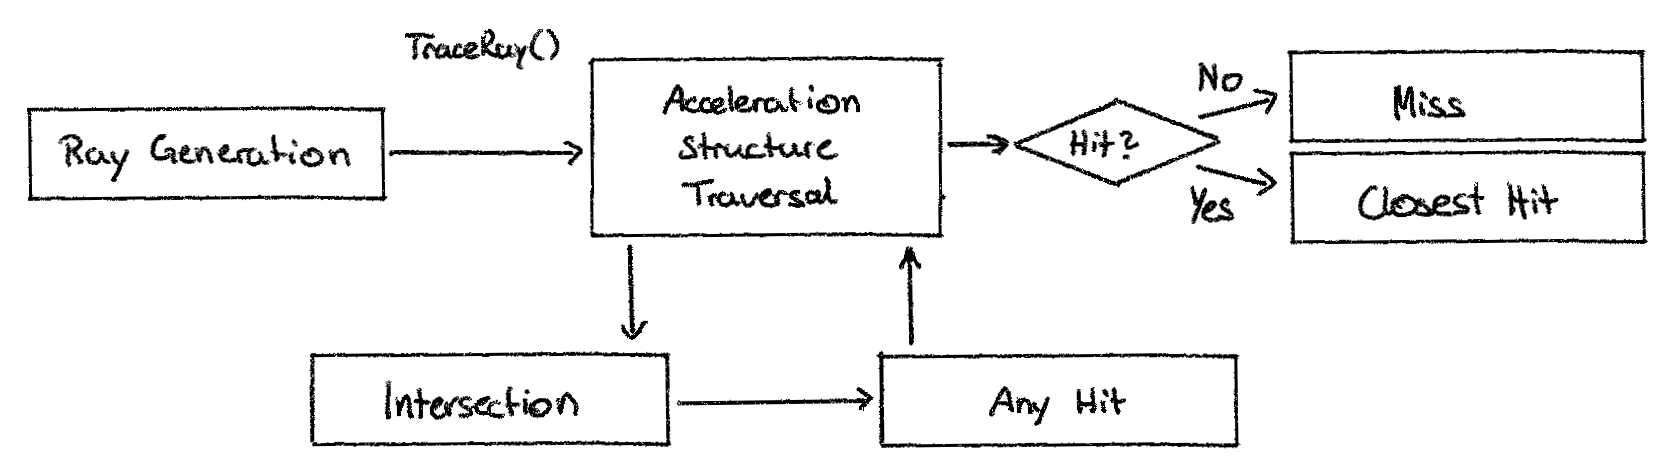
\includegraphics[width=\textwidth]{optix-kernel.png}
    \end{center}
    \caption{optix pipeline \cite{nvidia_nvidia_2022}}
    \label{fig:optix-kernel}
\end{figure}

The \textit{ray generation} program is the entry point of the device execution.
One uses a particular host code function to initiate the device-sided execution.
From here on, one can call additional functions to build an execution sequence.

A \textit{intersection} program is necessary for the acceleration structure traversal.
OptiX performs intersection tests during the traversal, using the program's implementation.
There is native support for triangle, curve and sphere primitives.
However, one can extend it with custom primitive types.
Note that OWL forms, on top of it, an abstraction for minimum expenditure.

The last two required programs are the \textit{closest hit} and \textit{miss} program.
The names are self-explanatory, but for completeness, one will mention them.
A \textit{closest hit} program gets called if a traced ray has one or multiple intersection points, providing the nearest intersection.
One can access information about the intersection point and the corresponding object inside the program.
A \textit{miss} program gets called if a traced ray has no intersection.
Note that both have access to the data of the ray.
The execution of these programs starts after a completed traversal.

\section{Application Design}

This section intends to give a general overview of the application, where one describes the individual tasks.
Furthermore, one will walk through some essential points that shaped the application.

One begins with a host-only functionality, loading mesh and material data.
Three-dimensional meshes have different representations and need corresponding loaders to bring the vertex normal and position data to memory.
Besides that, these representations can also contain information about the material data.
Accordingly, large libraries can load many file formats.
However, it seemed to be convoluted, and thus one decided to use the OBJ format because of its simplicity.
Another argument for that format was that all object vertices are in global coordinates; therefore, one has not had to handle transforms.
The normal and UV data are also optionally available.
For materials, one only needed a simple format to represent the Disney parameters' values and the object's corresponding name.
Hence, one decided to use the JSON format.

The next consideration is the exchange of data (host-device communication) and where the data should be available.
OptiX offers two strategies.
The first is the so-called SBT or shader binding table.
It allows the programmer to bind specific data to a program of the OptiX pipeline.
An essential difference to the second option is that the data will only be available to the designated program.
The second option is to create global constants that make the data available everywhere in the device.
For this thesis, the critical attribute is clarity.
Creating a global constant containing any data required during the renderer's lifetime is the easiest choice, making user-defined data types obsolete to a certain extent.

The next point is the path tracing itself, especially if one selects a recursive or iterative implementation.
Accordingly, the tasks of the programs, \textit{closest hit} and \textit{ray generation} change.
Intuitively, a recursive implementation would be the most straightforward approach because one described path tracing as a recursive formula.
However, one chooses an iterative implementation because the path construction is more apparent, and the procedure is easier to understand.
Hence, the implementation will be in the \textit{ray generation} program.

One summarises the different decisions to demonstrate how these interoperate in the application.
The host-sided application loads all required data for the path tracer, initialises with OWL the OptiX components and uploads the data to the graphics card.
Afterwards, one launches the rendering, and the host waits until the result is available through a host device buffer.
The launch causes an invocation of the \textit{ray generation} program for every pixel, which controls the calculation of paths that have a vertex on the camera plane associated with the corresponding pixel.
The \textit{closest hit} and \textit{miss} programs set the necessary state that allows the path tracer to load the mesh data in the device-sided path tracing routine through a global constant.
After the device has finished all calculations, the host can read the result and write it to a predefined destination.

\section{Colours}

Early, one expressed light as a quantum object where the energy consists of a constant and the frequency.
With a particular frequency present in light, one can determine a wavelength $\lambda$ that can describe colour in the light's visible spectrum.
The visible spectrum is a continuous infinite range of wavelengths, and light represents all wavelengths equally with the correct emitter.

The problem with such an infinitely large quantity is that computers cannot represent such ranges.
Accordingly, one has to perform quantisation and limited values.
Hence, it is crucial to select an appropriate colour model to represent a wide range of colours and provide a primitive to convert these values representable by computer monitors.

Nonetheless, one does not aim to employ a sophisticated colour model because of the required knowledge in colour theory and radiometry to understand such a model.
That is why one chooses simple RGB values to describe the different colours.
One knows that working with these values is inaccurate but sufficient for this thesis.
Note that it benefits three-component vectors to represent these colours.

Keep in mind that this topic becomes very complex because it is not only about accurately depicting light.
One has to account for human perception.

\section{Path Construction Routine}

The path construction routine builds the core of a path tracer.
It governs the strategy of finding vertices.
One mentioned early that the path tracer has a local sampling strategy that utilises ray tracing.
The following will present the individual parts of the routine; see appendix alg.~\ref{alg:path-construction}.

\subsection*{State}

The state of a path is necessary to determine the colour of a pixel.
One identified three metrics that control a path's contribution to a pixel.
Accordingly, one will define these metrics.

Radiance is a quantity from physics describing the relation of energy to a solid angle and projected area.
For paths, it will be the energy that a pixel on the camera plane could potentially receive.
One sets the radiance of a path through light sources, which are surfaces that emit light or the environment.
For this purpose, one retrieves the colour of the light and adjusts it with a constant of proportionality.
The throughput attenuates the potential received energy which yields the received energy.
One uses the eq.~\ref{eq:path-throughput} to track the state correctly.
The correct state remains valid as long as the values that update the throughput have not degenerated.
If one does not handle these values, then the throughput will be in an invalid state, causing image artefacts.
The last state is the path's depth, which describes the number of segments with one vertex on the camera plane and another on a light source.
It correlates to the throughput as the value potentially decreases with every added dimension.
Thus, one can interpret that paths with a high depth count contribute less to the result.

\subsection*{Ray Casting}

Ray casting is the selected method to find vertices for a path.
For this, one uses a ray $r(t)$ starting from a point $\vec{a}$ and sends it in the direction $\vec{b}$ to find an intersection point.
The application tests the ray against the geometry's acceleration structure, and one uses the \texttt{TraceRay} function to initiate the procedure.
One can pass a user-defined data type as a ray payload to access the intersection and object data.
The ray payload can hold any data required for the following steps.

\begin{align*}
    r(t) = \vec{a} + \vec{b} \cdot t
\end{align*}

The selected method is not mandatory because the selection of a surface point can happen arbitrarily.
Hence, one could potentially employ a method that randomly selects a point in the scene.
The major drawback is that segments are not always valid, leading to additional tests to verify the visibility.
Using ray casts to find vertices will invariably result in valid paths.
To relate that to the geometric term eq.~\ref{eq:geometry-term}, the visibility term $V(x \leftrightarrow x')$ will be equal to one, simplifying the equation correspondingly.

Refining the current method can positively impact performance and visual fidelity; see bidirectional path tracing.
Another possible extension is to use ray cast for other visibility tests, like shadow rays, to test for a light source occlusion, enabling multi-importance sampling.

\subsection*{Intersection Cases}

The next step in path construction is handling three intersection cases.
For this, one will distinguish between ray hit and miss, and in the case of a hit, one will refine the distinction between surfaces or lights.
One will start with the ray miss case, followed by the light hit case and finalised with a regular hit.

The ray miss case is straightforward to handle.
Because of no intersection, the path must terminate, and one must update the current path's radiance.
Depending on available options, one samples an environment map or uses a uniform colour and multiplies it with an intensity factor.
After the radiance calculation, one terminates the path construction by breaking the loop due to the iterative implementation.
For a recursive implementation, it would have been a return.

The light hit case is similar to the first case.
One can assess the material data through the ray payload to get the emission strength.
The emission strength is a constant value across the area of the light.
Accordingly, the radiance is equal to the emission strength.
Note that one did not sample the light; thus, there is no special handling of the probability density required; see eq.~\ref{eq:path-throughput}.
After one has updated the radiance, the path terminates.

A regular hit causes the routine to continue with the sampling and then repeats the construction loop.
One accesses material, mesh and ray metadata through the ray payload for the sampling and provides variables for the following steps.

\subsection*{Sampling}

This step determines the further course of a path.
One uses a material sampler to get all relevant information (reflectance, probability density and incoming direction) for the upcoming iteration and updates.

The sampling uses local shading coordinates; \cite{pharr_physically_2017}.
It requires converting the outgoing direction provided by the ray data from global coordinates to the local shading coordinates.
It also means that one has to conduct a transformation of the sampled incoming direction to global coordinates.

\begin{figure}[h]
    \begin{center}
        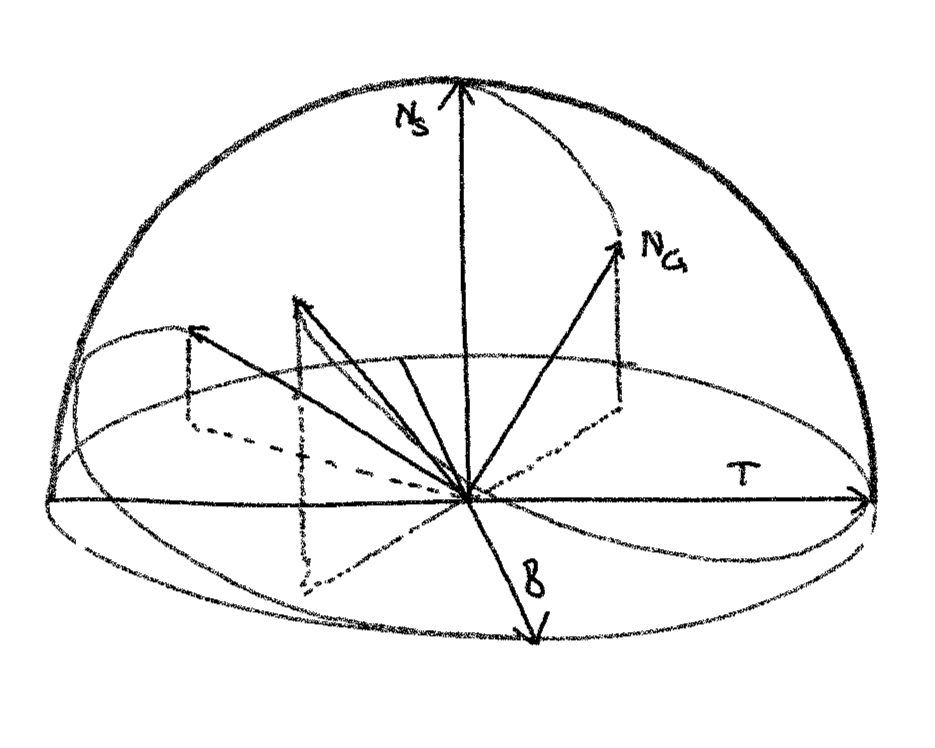
\includegraphics[width=0.4\textwidth]{local-space-coordinates.png}
    \end{center}
    \caption{local shading space coordinates}
    \label{fig:local-space}
\end{figure}

Next, one will elaborate on how to achieve the conversion and why it is beneficial.
The idea is that one can construct with the geometric normal $N_G$ a basis in the vector space $\mathbb{R}^3$ so that there are three orthogonal vectors in global coordinates.
The other basis describes the shading coordinates with a shading normal $N_S = (0,0,1)$ and the corresponding tangent and bitangent for the other axis.
Note that one does not need the shading coordinates for the light calculations, but they help make formulas more straightforward and explicit for computations.
For example, in the formula, $\cos(\theta_{\vec{v}})=v.z$, the cosine is the Z-component of the vector.

\subsection*{Random Termination}

The last step in the path construction is the Russian Roulette.
This function uses throughput and randomness to determine whether the path should terminate early and thus not contribute to the final result.
Notably, a small throughput should favour termination to reduce calculations for values with a minimal effect on the image's appearance.

\section{Disney Routines}

Throughout the two publications \cite{burley_physically_2012} \cite{burley_extending_2015}, Disney gave information regarding material observations and results and used models for light responses.
Regardless, they did not explain everything, leaving some points open for interpretation.
One compensated for the lack of information with other papers and other open source implementations.
Besides that, the most challenging part is to have a strategy implementing the Disney BSDF illumination model.
The strategy was to implement every lobe of the illumination model separately.
This separation allowed one to assess the surface responses of the individual lobes.
The assessment had a loose form, so no formal verification proved the correctness.
Nonetheless, the separate implementation leads to the fact that every lobe has its routine to evaluate reflectance and probability density function using a pair of incoming and outgoing directions.
In addition, there is a sampling routine that samples an incoming direction and encapsulates the evaluation.
Accordingly, one constructed the Disney BSDF sampling routine with all lobes implemented.
The following will elaborate on the mentioned points.

\subsection*{Light Lobes}

This section will present thoughts and observations rather than an implementation.
Note that implementation depends on the underlying algorithm and further required features.

For the lobes, one primarily oriented the implementation on the provided equations and references in the Disney papers.
One included all references in the appendix \ref{app:references} used for the implementation.
Additionally, one examined the source code of other renderer's implementations for unclear sections not explained by other references.
It is vital to be mindful of adopting concepts of other renderers because they do not necessarily fit into the rendering framework.
A fascinating observation was that every renderer handled sampling and evaluation differently.
Most of the \texttt{C++} implementations followed an OOP pattern, whereas some had a functional approach or a custom adaptation.
This variety, in general, made it difficult to derive a coherent implementation, and one can summarise that there is no defacto standard for a material implementation with a corresponding path tracer.

\subsection*{BSDF Sampling}

The sampling of the Disney illumination model turned out to be more difficult than expected compared to the lobes.
They have an illustration (fig. 4 \cite{burley_extending_2015}) that gives an idea of how to combine the lobes.
For more optimisation in the implementation, they decided on a unified model that blends in between the different models rather than one general model; \cite{burley_extending_2015}.

The problem is that no explanation or source code elaborates on the method to combine these different models.
Therefore, one analysed the other renderer's implementations.
The result is two concepts that one could potentially use.

The first option is to combine the lobes' routines, which means evaluating and mixing the lobes' values (reflectance and probability density).
However, when doing this, one has to be careful with the quantities, as averaging is not always doable.
Further, it gets incomprehensible with extensions or changes.

The second option is a more straightforward approach.
One derives probabilities for the lobes through the material values.
With these probabilities, one constructs a cumulative distribution so the application can use a random number between $[0,1]$ to select the lobe to sample, which mix materials more intuitively.

% \begin{table}[h]
%     \begin{center}
%         \begin{tabularx}{0.9\textwidth}{
%                 | >{\raggedright\arraybackslash}X
%                 | >{\raggedright\arraybackslash}X
%                 | >{\raggedright\arraybackslash}X |}
%             \hline
%             \textbf{Aspect}     & \textbf{Option A}        & \textbf{Option B}                   \\ \hline
%             \textit{sampling}   & per lobe                 & combined                            \\ \hline
%             \textit{evaluation} & per lobe                 & combined                            \\ \hline
%             \textit{mix}        & random selection of lobe & averaging values (reflectance, pdf) \\ \hline
%         \end{tabularx}
%     \end{center}
%     \caption{sampling strategies}
% \end{table}
